\subsection{CRUD}

The main focus of this sprint was to get the server up and running for the other layers. 
As we already had a working database, the goal of this increment was to write a CRUD API in C\# such that the other layers could use to access the database via HTTP requests.
The CRUD operations we implemented are based on requests from the other layers, and what they thought they needed to retrieve from the database.

To implement this, we split the CRUD operations into three different APIs handling different aspects of the database. 
The pipeline for these APIs is outlined in figure \ref{Node02Sprint3}.

\begin{figure}[h]
    \centering
    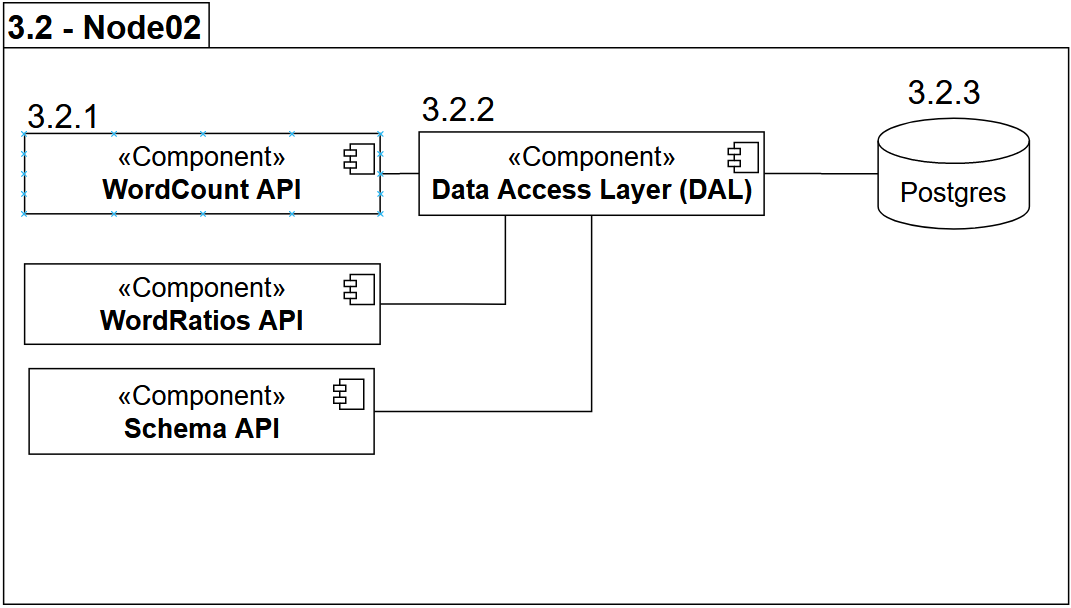
\includegraphics[width=\linewidth]{Images/Node02Sprint3.PNG}
    \caption{Node02 server pipeline in sprint 3.}
    \label{Node02Sprint3}
\end{figure}

\subsubsection{WordCount API}
The first API we created was the WordCount API in which we implemented two \texttt{GET} methods.
The first method called \texttt{GetAll} retrieves all words currently stored in the database.
The other \texttt{GET} method, simply called \texttt{Get}, takes a word as an argument and checks whether that word already exist in the database.
In the WordCount API, we also implemented a \texttt{POST} method called \texttt{Post} which takes a JSON object from the HTTP body as a parameter. 
The JSON object should correspond to an array of articles which will then be posted to the database. 

Before posting the data to the database, the method checks whether the article title, file path or words already exists in the database, and whether the input matches the JSON schema from the database.


\subsubsection{WordRatios API}
The WordRatios API is a view used by layer 4 to fetch specific data from the database.
As it is a view, it cannot be used to store new data. 
The primary purpose of the WordRatios API is to check how many times a given word occours in an article.

The API consists of two \texttt{GET} methods. 
The first method \texttt{GetAllWordRatios} is used to get all the entries in the WordRatios table.
The second method \texttt{GetMatches} is used to query one or more specific words. 
One may provide one or more sources in which to search for the specified words.
If no sources are provided, the database searches for the given words in all sources.

\subsubsection{Schema API}

The last API we implemented in this iteration is the Schema API which is used to post a JSON schema to the database, which is later used to verify JSON objects.
The route to this endpoint is simply \texttt{/Schema}. 
The body of the post request must consist of two fields - the schema name, which is its primary key in the database, and the schema content itself. 
A schema gets stored in the database in the format known as \texttt{jsonb} or JSON binary which is a built-in type provided by \postgres{}.
This format is used to store a JSON object as binary which uses much less space than a varchar or regular JSON type would.

\todo{Mention earlier that the database was accesed directly, instead of through an API}
\todo{Describe the structure of the database}

We chose not to implement the update and delete operations in this increment as it was not strictly needed to make the search engine work.
However, we have discussed doing so in a future increment.